\documentclass{article}

\usepackage[utf8]{inputenc}
\usepackage[margin=2cm]{geometry}
\usepackage{amsfonts,amsmath,amssymb}
\usepackage[T1]{fontenc}
\usepackage[french]{babel}
\usepackage{array}
\usepackage{url}
\usepackage{graphicx}
\usepackage{tikz}
\usetikzlibrary{arrows,automata,shapes}
\usepackage[nottoc,notlot,notlof]{tocbibind}
\usepackage{caption}
\usepackage{minted}
\usepackage{fancybox}
\usepackage{fancyhdr}
\usepackage{hyperref}
\usepackage{pgfgantt}


\pagestyle{fancy}
\fancyhead{}
\fancyfoot{}
\fancyhead[L]{\slshape \MakeUppercase{ACTING SHOOTING STAR}}
%\fancyhead[R]{\slshape Ismail ELOMARI ALAOUI - Nicolas LE QUEC - Vincent RIDACKER - Alexandre GISSAUD }
\fancyfoot[C]{\thepage}
\fancyfoot[R]{\slshape Encadré par: Sylvain Lombardy  }
\fancyfoot[L]{\slshape I1-P6-Groupe 2}
\renewcommand{\footrulewidth}{1pt}
\parindent 0ex
\renewcommand{\baselinestretch}{1,5}
\newcommand{\tikzlogo}{Ti\emph{k}Z}
\usepackage{color}
\usepackage{listings}
\definecolor{darkWhite}{rgb}{0.94,0.94,0.94}
 
\lstset{
  aboveskip=3mm,
  belowskip=-2mm,
  backgroundcolor=\color{darkWhite},
  basicstyle=\footnotesize,
  breakatwhitespace=false,
  breaklines=true,
  captionpos=b,
  commentstyle=\color{red},
  deletekeywords={...},
  escapeinside={\%*}{*)},
  extendedchars=true,
  framexleftmargin=16pt,
  framextopmargin=3pt,
  framexbottommargin=6pt,
  frame=tb,
  keepspaces=true,
  keywordstyle=\color{blue},
  language=C,
  literate=
  {²}{{\textsuperscript{2}}}1
  {⁴}{{\textsuperscript{4}}}1
  {⁶}{{\textsuperscript{6}}}1
  {⁸}{{\textsuperscript{8}}}1
  {€}{{\euro{}}}1
  {é}{{\'e}}1
  {è}{{\`{e}}}1
  {ê}{{\^{e}}}1
  {ë}{{\¨{e}}}1
  {É}{{\'{E}}}1
  {Ê}{{\^{E}}}1
  {û}{{\^{u}}}1
  {ù}{{\`{u}}}1
  {â}{{\^{a}}}1
  {à}{{\`{a}}}1
  {á}{{\'{a}}}1
  {ã}{{\~{a}}}1
  {Á}{{\'{A}}}1
  {Â}{{\^{A}}}1
  {Ã}{{\~{A}}}1
  {ç}{{\c{c}}}1
  {Ç}{{\c{C}}}1
  {õ}{{\~{o}}}1
  {ó}{{\'{o}}}1
  {ô}{{\^{o}}}1
  {Õ}{{\~{O}}}1
  {Ó}{{\'{O}}}1
  {Ô}{{\^{O}}}1
  {î}{{\^{i}}}1
  {Î}{{\^{I}}}1
  {í}{{\'{i}}}1
  {Í}{{\~{Í}}}1,
  morekeywords={*,...},
  numbers=left,
  numbersep=10pt,
  numberstyle=\tiny\color{black},
  rulecolor=\color{black},
  showspaces=false,
  showstringspaces=false,
  showtabs=false,
  stepnumber=1,
  stringstyle=\color{gray},
  tabsize=4,
  title=\lstname,
}

\begin{document}


\begin {titlepage}
  \begin{center}
      \vspace*{1cm}
    \Large{\textbf{Acting Shooting Star}}\\
    \Large{\textbf{Rapport de projet}}
    \vfill
    \begin{figure}[h]
        \centering
        
\includegraphics[scale=0.5]{MATMECA.PNG}
    \end{figure}
    \vfill    
    
    %\line{1,0}{400}\\[1mm]
    \huge{\textbf{Projet de programmation - S6}}\\[3mm]
    \Large{\textbf{-- I1 - ENSEIRB-MATMECA --}}\\[1mm]
    \Large{\textbf{Encadrants: M. David RENAULT - M. Sylvain Lombardy  }}\\[1mm]    
    %\line{1,0}{400}\\
    \vfill
    Par Ismail ELOMARI ALAOUI - Nicolas LE QUEC - Vincent RIDACKER - Alexandre GISSAUD\\
    \today\\
  \end{center}
\end{titlepage}



 \tableofcontents
%\thispagestyle{empty}
\clearpage
\newpage

\section*{Introduction}
    \subsection*{Contexte}
    Ce rapport a pour objectif de décrire l’ensemble du processus de réalisation d'un projet de programmation basé sur le langage Scheme ($Drracket$). Ce projet est conçu par Mr. David RENAULT, le directeur des projets à l'ENSEIRB-MATMECA, pour aider les élèves en première année d’informatique à avoir des compétences basiques voire avancées sur l'utilisation du scheme. Le projet consiste en l’implémentation d'un jeu appelé ACTING SHOOTING STAR, en racket. Nous sommes guidés par les questions produites dans le projet, afin de premièrement bien structurer le projet, et ensuite implémenter des acteurs puis un monde. Enfin, nous devons animer le tout à l'aide de 2 importantes bibliothèques: $Luxx$ et $Raart$.

    \subsection*{Description du sujet}
  Ce projet nous amène dans un monde virtuel dans lequel nous sommes un joueur (un acteur), qui essaie d'éviter certes l'embouteillage causé par d'autres acteurs mais aussi leurs missiles. Cet acteur n'est pas non plus sans espoir, il peut se protéger en tirant ses propres missiles, face aux ennemis malveillants. Ce projet est  inspiré par le travail de  C. L. Webber $Terminal$ $Phase$, dans lequel un modèle basé sur les acteurs est utilisé.
  \\
  L'implémentation de ce modèle provoque plusieurs problématiques:
  \begin{itemize}
    \item Comment un acteur peut-il être proprement structuré?  
    \item Comment ce monde virtuel que nous souhaitons codé, peut-il lui-même être structuré? 
    \item{Comment les acteurs communiquent-ils entre eux ?}
    \item Et, comment peut-on joliment animer ce monde saturé par des acteurs qui entre-échangent des messages? 
    \end{itemize}
  Ce sont de façon relativement succincte, les consignes principales à résoudre et à respecter pendant notre projet.
\newpage
 


 \section{Méthode de travail}
    \subsection{Répartition des tâches}
    Tout d'abord, notons que ce projet a été du début à la fin un travail d'équipe complet, dans lequel nous avons appris tout du long à beaucoup échanger et à travailler ensemble, tout en se répartissant les tâches quand cela était nécessaire. Nous pensons que tous ce qui peut fracasser une équipe de programmeurs est la mal-structuration du projet. Nous pensons avoir fait de notre mieux pour éviter cette catastrophe.
    
    Pour s'organiser, nous nous rejoignions en vocal sur Discord généralement. Lorsque nous sommes d'accord sur les tâches à réaliser et leur répartition, nous commençons à coder. Dès qu'une tâche est finie ou que quelqu'un a besoin d'aide, on propose de nouvelles fonctionnalités à implémenter ou l'on aide quelqu'un qui aurait besoin de soutien.
    Nous nous connectons en vocal chaque séance pour coder ensemble et être disponible directement si une question se posait mais aussi pour combattre la solitude du programmeur.
    
    \subsection{Thor Project}
    Nous avons utilisé la Forge (le serveur $Thor Project$) de l'ENSEIRB-MATMECA pour gérer les différentes versions de notre projet. L'évolution du projet visible sur cette Forge peut mettre en évidence nos progrès en tant que débutants programmeurs sur Scheme.\\
    Les codes sources, évidemment présents sur la forge, ont été codés à l'aide de l'application $Drracket$ v7.6. Nous vous prions de vérifier votre version avant d'exécuter le jeu.\\
    Nous avons utilisé comme il nous l'avait été demandé LaTeX pour rédiger ce rapport. Afin de simplifier le travail simultané sur l'écriture de ce rapport, nous avons utiliser $Overleaf$, un éditeur LaTeX en ligne.\\

    \subsection{\textit{Makefile}}
Nous avons utilisé l'outil d'aide à la compilation \textbf{$make$}, en réalisant un \textbf{$Makefile$}.
L'exécution du jeu est très simple. Il suffit d'écrire la commande suivante:
\textit{make}. Une fenêtre du jeu apparaîtra dans le terminal sur laquelle vous pourrez jouer instinctivement (\textit{ZQSD} pour se déplacer, \textit{ESPACE} pour tirer, \textit{A} et \textit{E} pour se déplacer dans le temps, \textit{P} pour mettre le jeu en pause et \textit{T} pour quitter le jeu). Il est possible d'ajouter l'option \textit{-f <nb>} pour choisir le nombre de fps du jeu.
\\ Afin d'approuver la validité de nos implémentations et de nos fonctions, plusieurs tests ont été programmés. Pour les exécuter, écrivez la commande suivante: 
\textit{make test}. \\ Enfin, la commande \textit{make doc} permet d'afficher la documentation de la bibliothèque dans votre navigateur. Dans celle-ci est présent les descriptions des fonctions utiles à l'utilisateur pour concevoir son jeu ainsi que des explications pour comprendre le fonctionnement de la bibliothèque.

    \subsection{Architecture du répertoire $GIT$}
    Notre dépôt contient plusieurs répertoires: $"src"$ qui contient tous les codes sources utilisés pour passer les tests et créer ce magnifique monde virtuel. Et le répertoire $"doc"$ qui contient la documentation du projet.
    Cette documentation est générée à l'aide du fichier $actors.scrbl$, présent -espérons- sur notre dépôt. La méthode de production des fichiers de documentation est expliquée dans la sous-section précédente. Enfin, le répertoire $"report"$ contient ce rapport en version $pdf$ et en \LaTeX (code source).

\newpage

\section{Structuration du projet}
\subsection{$Actor$}
Dans le cadre de ce projet, un message est une liste constituée d'un \textit{tag} (un symbole), d'une fonction ainsi que d'un ensemble quelconque de paramètres (par ex. (list 'player move 1 0)). Un acteur est simplement une structure de données possédant un état propre, et capable de recevoir et d'émettre des messages. En fonction des messages qu'il reçoit, il peut choisir de mettre à jour son état, d'émettre de nouveaux messages, voire même de créer de nouveaux acteurs ou de mourir de sa plus belle mort.
La structure principale d'un $actor$ est donc très claire. Mais, d'autres champs ont été ajoutés pour mieux s'adapter à certaines situations. Nous avons pensé implémenter des événements particuliers qui rendront le jeu plus actif et plus aimable. Par exemple, un évènement o\'u tous les acteurs ennemis tirent à la fois, ou un autre o\'u la vitesse des murs fluctuent pendant un moment, mais également l'implémentation de quelques compétences pour le joueur. \textit{(Petit Scénario: Après avoir tué 10 ennemis, le joueur obtient une compétence qui lui permet d'être invincible pour quelques instants. Le joueur peut manuellement l'utiliser en cliquant sur 'x' par exemple)} et pourquoi pas un combat avec un \textit{boss}). Ces réflexions nous ont mené à ajouter un champ \textit{tag} à l'acteur. Ce champ lui offre une identité (\textit{wall}, \textit{missible},  \textit{player}, ...) . Sa position précédente \textit{prev-pos} est nécessaire pour l'implémentation de certains messages (ex. \textit{collide}).
Le champ \textit{msg-next-tick} sert à stocker les messages qui seront envoyés à l'acteur au prochain \textit{tick}. Il est notamment utilisé lorsque les acteurs veulent s'envoyer des messages à eux-même (pour ne pas générer de boucle infinie).
L'attribut \textit{collide} est une fonction qui gère le résultat d'une collision de l'acteur avec un autre. Elle ne détecte pas les collisions mais uniquement leurs conséquences sur l'acteur.
Le champ \textit{attributes} est un attribut particulier de la structure. Il ne possède aucune spécification de format et est par conséquent, complètement libre en terme de structure. Il est libre d'utilisation par son acteur. Ce champs peut être utilisé par exemple pour stocker les points de vie du joueur ou les dégâts d'un missile.
(cf. Figure \ref{fig:actor})
  \begin{figure}[h]
      \centering
        \begin{verbatim}
            (struct actor (pos prev-pos mailbox msg-next-tick tag collide sprite attributes))
        \end{verbatim}
      \caption{Structure $actor$}
      \label{fig:actor}
  \end{figure}
  
\subsection{Messages}

\subsubsection{Description}

Les messages concernés ici sont ceux destinés aux acteurs. Ils sont envoyés dans leur \textit{mailbox} pour être lu et interprétés. Les messages sont une liste dont le premier paramètre est le \textit{tag} du destinataire, le second une fonction d'un format spécifique (cf \ref{ref:fonction-message}) et vient ensuite un nombre quelconque d'arguments pour la fonction. Ce format a été choisi pour donner à ces fonctions le plus large champ d'action possible. La fonction s'appliquera à l'acteur ayant reçu le message. De ce fait dans le message, le paramètre acteur ne sera pas spécifié pour la fonction. 

Par exemple, imaginons une fonction \textit{move} prenant en paramètre un acteur et deux nombres x et y. Le message envoyé à un acteur avec le \textit{tag} \textit{player} pour le déplacer sera : (list 'player move 1 2).

Plus généralement on obtient la spécification suivante pour les messages:

\begin{figure}[h]
      \centering
        \begin{verbatim}
            (list tag fonction-message arg1 arg2 ... argN)
        \end{verbatim}
      \caption{Structure d'un $message$}
      \label{fig:struct-message}
  \end{figure}

\subsubsection{\label{ref:fonction-message} Fonctions des messages}

Les fonctions contenues dans les messages ont une importance particulière dans ce projet. Elles seront appelées \textit{fonction d'actions} dans la suite de ce rapport.

Ces fonctions prennent nécessairement un acteur en premier paramètre et renvoie en sortie une paire dont le premier élément est une liste d'acteurs et le second une liste de messages. Elles peuvent prendre autant de paramètres supplémentaires qu'elles le souhaitent tant que le premier est un acteur.

Ces fonctions déterminent une transformation appliquée à un acteur. La liste d'acteurs en sortie est la liste des acteurs toujours "en vie" et/ou créés après application de cette fonction et la liste des messages en sortie sera redistribuée aux acteurs concernés suivant leur \textit{tag} (ce sont les mondes, structure \textit{world}, qui se chargeront de cela).
Il faut noter que ces fonctions interviennent au niveau de l'acteur. Le résultat de cette fonction ne détermine pas l'ensemble de tous les acteurs toujours en vie dans le jeu mais uniquement l'ensemble des acteurs toujours en vie après l'application de cette fonction sur l'acteur concerné.

\begin{center}
    \begin{verbatim}
    (define (kill act) (cons '() (list (list 'bullet kill))))
    \end{verbatim}
\end{center}
    
Ainsi la fonction ci-dessus appliquée à un acteur ne renverra pas cet acteur le tuant et renverra un seul message destiné aux acteurs avec le tag \textit{bullet}.
    
\subsubsection{Exemple d'application}

Les fonctions d'actions sont très libres dans leurs applications grâce au format définie pour elles. Elles ne peuvent que créer des acteurs et des messages en plus d'accéder à l'acteur qu'elles prennent en paramètre. Cependant, cela suffit à obtenir des comportements plutôt intéressants. En exploitant la capacité des fonctions de messages à envoyer un message au prochain \text{tick} à l'acteur qui les appelle, on peut créer des fonctions qui se déroule sur plusieurs \textit{ticks}. On peut notamment citer la fonction \textit{tick-counter} qui permet d'appliquer une fonction de message avec ses paramètres après un certain nombre de \textit{ticks} passés. Pour ce faire, le message garde un compteur de \textit{tick} comme paramètre et se renvoie lui-même à l'acteur au prochain \textit{tick} en incrémentant le paramètre comptant les \textit{ticks} (un acteur peu s'envoyer un message à lui-même grâce à la fonction \textit{actor-send} prenant un acteur et un message comme argument). La fonction \textit{tick-counter} utilise une structure \textit{event} qui contient la fonction à appeler, à partir de combien de \textit{ticks} et avec quels arguments.

En utilisant ce genre de fonction, on peut créer des actions continues sur le temps. Par exemple, le jeu contient un type d'ennemi "UFO" qui suit une succession de mouvement : il se déplace horizontalement, tire puis se déplace verticalement.

La fonction \textit{tick-counter} n'est pas la plus efficace pour compter les \textit{ticks} (car on ajoute un compteur pour chaque message de contenu \textit{tick-counter} et fonctionne plutôt comme un compte à rebours. Elle permet de créer des niveaux scénarisés, cependant pour son bon fonctionnement, il faudrait déterminer les actions devant s'effectuer à chaque tick. Ce qui n'est pas le plus pratique.

En utilisant le principe de \textit{tick-counter}, on peut alors créer des fonctions comme \textit{repeat-call-delayed} qui permettent d'élaborer des messages qui rappellent des fonctions indéfiniment suivant une période définie. C'est en utilisant ce genre de fonction que le projet contient des générateurs automatiques d'ennemis.

\subsection{\textit{World} et \textit{Runtime}}
   Rappelons que l'objectif de ce projet consiste à mettre en place une bibliothèque d'acteurs afin de construire un jeu ressemblant à un \textit{shoot'em up}. Pour simplifier par rapport au modèle de programmation cité ci-dessus, nous allons considérer que les acteurs se mettent à jour de manière synchronisés. Une horloge globale découpe le temps en intervalles (\textit{tick} en anglais). Au début d'un intervalle de temps, les acteurs n'ont aucun message en attente. Ils reçoivent un ensemble de messages pendant cet intervalle (\textit{move}, \textit{collide} ...) sans autre modification. Ces fonctions peuvent leur être envoyées par d'autres acteurs, par eux-même, ou même par le \textit{runtime} (qui sera détaillé juste après). A la fin de l'intervalle de temps, ils vident leur boîte de message et se mettent à jour en fonction de ce qu'ils ont reçu. Tout ce processus d'échange et d'interprétation des messages est géré par les \textit{worlds} mais la mécanique de l'horloge globale est réalisée à l'aide d'une structure de donnée globale, le \textit{runtime}, organisant la mise à jour simultanée de tous les acteurs. Les messages sont alors considérés comme reçus simultanément pendant cet intervalle. L'implémentation d'un monde (\textit{world}) et d'une horloge ou un contrôleur de temps (\textit{runtime}) était donc indispensable.
    \begin{figure}[h]
      \centering
        \begin{verbatim}
            (struct world (actors mailbox))
        \end{verbatim}
      \caption{Structure \textit{world}}
      \label{fig:world}
  \end{figure}
  \\
  Un monde contient 2 champs (cf. Figure \ref{fig:world}) : 
  \begin{itemize}
      \item \textit{actors} est une liste de listes. En effet, les acteurs sont regroupés dans des listes selon leur \textit{tag}. Le premier argument de chaque sous-liste commence par le \textit{tag} des acteurs de celle-ci. Exemple de liste d'acteurs : (list (list player a0) (list enemy a1 a2))   
      \item \textit{mailbox} est liste contenant les messages qui seront envoyés aux acteurs au prochain \textit{tick}.
  \end{itemize}
  
   \begin{figure}[h]
      \centering
        \begin{verbatim}
            (struct runtime (world-count max-worlds worlds functions))
        \end{verbatim}
      \caption{Structure $runtime$}
      \label{fig:runtime}
  \end{figure}
  
  Dans ce monde virtuel, des multi-dimensions sont tout à fait envisageables. Elles peuvent être modélisées comme des phases ou des stages du jeu. Le joueur passe d'un monde à un autre, s'il reste en vie à la fin d'une phase particulière. 
  
  De plus afin de permettre au joueur de revenir dans le temps pour pouvoir rejouer des séquences qu'il pense avoir échoué ou qu'il voudrait optimiser, les états des mondes sont sauvegardés à chaque \textit{tick} dans le \textit{runtime}. Remonter dans le temps revient alors à se balader dans cet liste de mondes. 
  (cf. Figure \ref{fig:runtime}):
  \begin{itemize}
    \item \textit{world-count} est le nombre de monde courant dans le \textit{runtime}.
    \item \textit{max-worlds} est le nombre maximal de mondes sauvegardés. Cela définit en quelque sorte la mémoire du \textit{runtime}.
    \item \textit{worlds} est une liste contenant tous les mondes sauvegardés. Le premier monde de la liste est le monde courant. 
    \item \textit{functions} est une liste contenant les fonctions primordiales au fonctionnement de la boucle de jeu. (ex. \textit{world-update}, \textit{world-empty-mailbox}, ... ) 
  \end{itemize}

La figure \ref{fig:boucle_jeu} résume le déroulement d'un \textit{tick}.

\begin{figure}
    \centering
    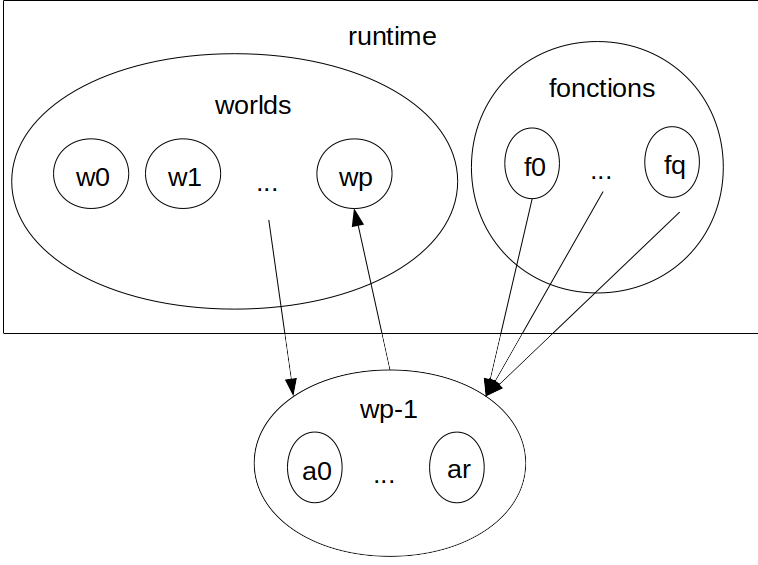
\includegraphics[scale=0.5]{img/boucle_jeu.png}
    \caption{Schéma de la boucle de jeu}
    \label{fig:boucle_jeu}
\end{figure}

Pour commencer, on récupère le monde courant et on lui applique toutes les fonctions du \textit{runtime}. Dans celles-ci est notamment présent la fonction \textit{world-empty-mailbox} vidant la messagerie du monde courant et envoyant les messages aux acteurs correspondant (en accordance avec le \textit{tag} des messages). Chaque acteur va ensuite effectuer les actions qui lui ont été envoyées et renvoyer une liste d'acteurs (créés et/ou en toujours en vie) ainsi qu'une liste de messages qui sera par la suite transféré dans la \textit{mailbox} du monde pour le prochain \textit{tick}. Une fois que tous les acteurs ont effectué leurs actions, l'état actuel du monde est affiché grâce aux bibliothèques \textit{raart et lux}. Pour finir ce nouveau monde ainsi obtenu est ajouté à la liste des mondes sauvegardés. Lorsque l'on arrive en limite de mémoire, le monde le plus ancien est supprimé. 

\subsection{Optique de l'architecture}

Ce projet consiste en l'implémentation d'un jeu en suivant un modèle basé sur des acteurs échangeant des messages. Pour ce faire, nous avons essayé de séparer les rôles et les responsabilités de chaque structure. Les structures agissent à différentes échelles de libertés :
\begin{itemize}
    \item Les acteurs ne peuvent accéder qu'à eux-mêmes. Ils ne peuvent pas modifier le \textit{world} ou le \textit{runtime}. Ils peuvent échanger des messages entre acteurs par l'intermédiaire du \textit{world}.
    \item Les mondes (structure \textit{world}) englobent les acteurs. Ils sont chargés de délimiter un périmètre dans lequel des acteurs sont libres d'agir (comme dans un vrai monde). Ils ont aussi la charge de jouer le rôle de la poste et de retransmettre les messages selon les \textit{tag} (les acteurs étant confinés, ils ne peuvent pas jouer le rôle du facteur).
    \item La structure \textit{runtime} fait office de superviseur des mondes. Elle assure le bon déroulement des mondes en appliquant des routines de fonctions (notamment \textit{world-update}) et fait l'interface avec l'utilisateur de l'application. Cette structure se charge également par conséquent des "retours dans le passé" à l'aide d'une liste de monde.
\end{itemize}

Pour faire tourner un monde, il faut des acteurs, mais il faut également que ces acteurs disposent d'actions. Nous avons ainsi décidé de maximiser la liberté de leurs actions comme dans un vrai monde. Ces actions sont modélisées à travers les messages et les fonctions d'actions. Les fonctions d'actions décrivent quelles conséquences à une action sur un acteur. Ce sont ces fonctions qui s'occupent de la plupart des interactions du jeu tandis que les structures \textit{world} et\textit{runtime} ne s'occupent que de maintenir les routines.
   
\section{Fonctions particulières}

\subsection{actor-update-list}

Cette fonction prend un acteur en entrée puis lit, applique et enlève tous ses messages pour enfin renvoyer le résultat dans le même format que les fonctions d'action.

Cette fonction a été particulièrement difficile à programmer en respectant le format des fonctions d'action et l'aspect fonctionnel du projet.
En effet, puisque les fonctions de messages renvoient simplement une liste d'acteurs, il n'est pas possible d'identifier lequel est l'acteur initialement passé en paramètres sans appliquer de contraintes sur les fonctions de messages (comme par exemple ne pas changer le \textit{tag} de l'acteur en entrée pour effectuer un test d'égalité à la sortie).
On ne peut pas non plus identifier l'acteur par sa position dans la liste sans créer un acteur "mort" spécifique servant à l'identification. 

De ce fait, la fonction \textit{actor-update-list} maintient une liste d'acteurs en vie, et met à jour tous les acteurs de cette liste qui ont des messages sans distinction. Pour ce faire, elle ajoute la liste des acteurs résultant de l'application d'un message sur l'acteur propriétaire à la liste des acteurs en vie et répète le processus tant qu'il reste des messages.

Par conséquent, toute fonction d'action qui créerait un acteur ayant un message dans sa \textit{mailbox} verra cet acteur mis à jour dans le même \textit{tick} que sa création. Pour pouvoir, envoyer des messages qui seront interprétés au prochain \textit{tick}, il a donc été nécessaire de mettre en place l'attribut \textit{msg-next-tick} dans \textit{actor} (servant en quelque sorte de \textit{mailbox} tampon).

\subsection{Animation et Affichage}

Pour l'affichage, le projet se base sur la bibliothèque Raart. Tous les acteurs disposent d'un attribut \textit{sprite} qui doit être affichable dans un terminal; il doit être du type \textit{raart}. C'est la structure \textit{runtime} qui s'occupe de cela, les acteurs décrivent seulement comment ils apparaissent et le \textit{runtime} les affiche. Pour cela, nous avons choisi de simplement afficher tous les acteurs du monde "courant" à l'aide de la fonction \textit{place-at} fournie par \textit{Raart}. C'est le rôle de la fonction \textit{(define (display-world world))} qui produit l'objet Raart qui sera affiché dans le terminal en regroupant tous les acteurs du \textit{world} passés en paramètre. 

\subsection{Collisions}

\subsubsection{Attribut collide dans la structure $actor$}

Cet attribut est une fonction du format des fonctions de messages (cf \ref{ref:fonction-message}). Ce choix a été fait pour permettre aux acteurs de gérer individuellement la conséquence d'une collision par eux-même. Lorsque le jeu détecte une collision entre deux acteurs, il envoie un message de collision aux deux acteurs concernés qui réagiront en conséquence.  On peut ainsi moduler un comportement différent selon chaque acteur.

\newpage
\section{Boucle principale}
Nous possédons maintenant tous les outils nécessaires à l'implémentation de la boucle de jeu dans le $src/main.rkt$. La boucle de jeu utilise les méthodes fournies par la bibliothèques Lux dans la structure \textit{runtime}.

A chaque \textit{tick}, la boucle appelle simplement la fonction \textit{runtime-apply-func} qui applique un ensemble de fonction à la structure \textit{world} courante. Cet ensemble de fonctions est stocké dans la structure \textit{runtime} et peut être modifié selon les besoins, mais certaines fonctions comme \textit{world-update} et \textit{world-empty-mailbox} sont ajoutées de base.

La gestion des contrôles utilise également Lux, lorsque l'on appuie sur une touche, la structure \textit{runtime} envoie un message correspondant aux acteurs concernés grâce à leur \textit{tag}.

La fonction \textit{word-output} de Lux est utilisée pour l'affichage. Dans ce projet, nous affichons le monde "courant" grâce à la fonction \textit{display-world}.

Le jeu s'arrête lorsque le \textit{runtime} ne détecte plus acteur possédant le tag \textit{player} dans le monde courant.

\section {Tests effectués}
Afin de s'assurer de la robustesse de nos structures ainsi que de la correction de nos algorithmes, nous avons tout au long du projet élaboré plusieurs tests à l'aide de la bibliothèque \textit{RackUnit}. La commande \textit{make test} exécute ces tests. Nous nous sommes concentré sur la robustesse absolue de notre code, en conséquence plusieurs tests permettent de vérifier la validité de nos fonctions même dans les cas les plus extrêmes: de la belle mort d'un acteur, à la malheureuse création d'un autre, à l'extraordinaire voyage entre les mondes en survivant aux dangereuses collisions entre acteurs de différents \textit{tags}, tout en passant par plusieurs positions pour enfin réaliser la \textit{démo} dont le \textit{gif} est sur la chaîne \textit{SLACK} "projets-s-actors-gif".
Comme prévu, tous les tests ont été programmés comme une application de plusieurs fonctions dans des scénarios o\'u nous connaissons les conséquences avant l'exécution.

\section{Conclusion}

\subsection{Programme et ses options}

\subsubsection{Code principal}
En exécutant le programme à l'aide de la commande \textit{racket src/main.rkt -f \%} en remplaçant \% par le \textit{fps} (\textit{frames per second}) voulu. Le \textit{fps}
est maintenue à 60 par défaut, le jeu peut être lancé avec cette valeur en écrivant la commande \textit{make}. 
Par exemple, l'utilisateur peut choisir l'option \textit{f} en utilisant la notation suivante dans le terminal: \textbf{racket src/main.rkt -f 10}. Si cette syntaxe n'est pas respectée, un message d'aide apparaît et l'utilisateur doit à nouveau taper la commande. Si les valeurs rentrées ne sont pas compatibles (par exemple, \textit{f<=0}), les valeurs par défaut sont utilisées. 

\subsubsection{Code de test}
En lançant la commande \textit{bash} \textbf{make test} dans le terminal, les codes de test sont directement compilés et exécutés. Il s'affiche alors à l'écran le nombre de tests réussis par catégorie de test, puis le nombre globale de tests réussis. 

\subsection{Difficultés rencontrées et retour sur expérience}
D'une façon très générale, ce premier projet en langage \textit{scheme racket} n'était pas exactement du même degré de facilité que les TDs de programmation fonctionnelle.
Nous comprenons que ce cours était basé sur les bases de \textit{racket}, mais la différence de difficulté entre les exercices résolus en TD et ce projet est énorme. Du coup, nous avons eu plusieurs problèmes, notamment sur la structuration du projet. 
De plus, le changement de façon de programmer entre un langage itératif et un langage fonctionnel a été difficile au début. Plutôt que de simplement affecter les instructions à la suite une par une, il a fallu programmer de sorte à ce que les changements s'effectuent et se cumulent à la suite. Nous pensons que le seul aspect itératif du projet est la boucle de jeu basé sur Lux.

De plus, il a été plus difficile de s'organiser à 4 plutôt qu'a 2 personnes, d'autant plus que nous n'étions pas familiarisé avec la création de jeu en racket (surtout la partie interface graphique et gestions des inputs). Il a fallu se concerter et comprendre ensemble le sujet pour définir des actions pouvant être faites en parallèles. Pour cela, nous avons dû définir l'architecture du projet en avance et notamment les formats des fonctions. Nous avons pu entrevoir à quel point il était embêtant de s'être trompé sur l'architecture lorsqu'il a fallu changer les formats des fonctions d'actions pour pouvoir renvoyer une liste de messages et une liste d'acteurs. Avec du recul, nous aurions peut être dû implémenter une structure \textit{message} mais nous avons eu cette réflexion trop tard dans le projet.

Nous pensons que l'un des aspects les plus problématique de ce projet a été de debugger. Les erreurs d'exécutions sont particulièrement compliquées à gérer notamment à cause du typage dynamique du langage (et probablement notre manque d'expérience). La mise en place de contrat a été d'une grande aide pour combattre ce fléau.

Enfin, le côté autonome dans la recherche quant à l'utilisation de \textit{raart} et de \textit{Lux} a été assez intéressant. Nous nous sentons maintenant plus enclins à utiliser des bibliothèques dans notre code. Nous avons aussi pu réaliser l'importance de la documentation et de la clarté des fonctions(pour qu'elles soient facile à identifier et à utiliser).

Pour résumer, nous laissions notre imagination couler(Implémentation de plusieurs mondes, combat contre des $boss$ , des événements ...), et c'est exactement cela qui a rendu ce projet plus difficile à programmer. Enfin, créer ce jeu était une expérience très appréciable, nostalgique. Et, nous trouvons que cette nostalgie des jeux du passé, la curiosité d'explorer des bibliothèques d'animation et d'affichage graphique et la compétitivité entre les groupes pour réussir à proprement lancer son jeu nous a certainement aidé à nous évader pendant cette pandémie. Ce projet nous a aidé à renforcer nos compétences dans le langage $scheme$, à développer notre esprit d’équipe et de collaboration, ce qui est pour nous une préparation essentielle à ce qui nous attend dans les années à venir, et a réanimé la passion, de certains d'entre nous, à créer des jeux vidéos. C'était pour cela un excellent projet à programmer malgré les conditions particulières du confinement et nous souhaitons qu'il soit aussi merveilleux à corriger.

\section{Remerciements}
Nous remercions tout d'abord M. David RENAULT pour les remarques, aides,  observations mais aussi la bonne humeur qui nous ont été données soit par \textit{SLACK}, soit par courriel, ainsi que pour l'élaboration de ce projet original. De plus, nous remercions M. Sylvain LOMBARDY, qui nous a accompagné tout au long du projet en nous encadrant et en répondant à toutes nos questions. Ses réflexions sur l'importance de la rigueur dans la programmation nous ont été utile pour ce projet et nous seront probablement utiles pour le reste de notre vie de programmeur. 

\section{Références}
\subsection{Internes}
\begin{itemize}
    \item \url{https://www.labri.fr/perso/renault/working/teaching/projets/}
    \item \url{https://www.labri.fr/perso/renault/working/teaching/schemeprog/schemeprog.php}
\end{itemize}
\subsection{Externes}
\begin{itemize}
    \item \url{https://docs.racket-lang.org/plait/Tutorial.html}
    \item \url{https://www.overleaf.com/}
\end{itemize}

\end{document}